% =====================================================================
%  附录 AT：波的传播——截止、共振与模式转换（注明出处）
%  数值唯一来源：tmp/appAT_calc.py（只 print，输出 tmp/appAT_calc.txt）
%  单位口径：SI；频率写成 GHz/MHz，长度写成 m/mm/um，密度写成 m^-3，磁场写成 T。
%  与其他附录的分工：附录 AS 管几何光学（本附录正好管它失效的地方：截止、共振、消逝层）；
%  附录 M 管加热与电流驱动（本附录只算波在哪里停、在哪里被吸收）；
%  附录 AQ 管干涉与相位、附录 AN 管偏振诊断；附录 AE 管动理学（本附录沿用它的热速度口径）；
%  附录 S/U 管约束与点火（本附录不重复功率账）。
%  版权口径：只复算、不复制原书表格与图；直接引用处写「不复制」并标出处。
% =====================================================================

\section{冷等离子体色散关系：介电张量记住了磁场}
\label{sec:app-at-tensor}

附录 AS 把波画成射线，代价是假装等离子体只是「折射率随位置变化的介质」。一旦波长不再远小于
不均匀尺度，或者波走到折射率趋于零、趋于无穷的地方，射线画法就失效了。失效的地方恰好是聚变
装置里最重要的地方：\textbf{截止层}（波被反射）与\textbf{共振层}（波被吸收或被转换）。

要看清这些，必须回到冷等离子体的介电张量。取 D1 工作点：中心密度
$n_\mathrm{e0}=1.0\times10^{20}$ m$^{-3}$、电子温度 $T_\mathrm{e}=9.194$ keV、轴上磁场
$B_0=5.3$ T、小半径 $a=2.0$ m，密度剖面 $n_\mathrm{e}(r)=n_\mathrm{e0}[1-(r/a)^2]$、
磁场剖面 $B(r)=B_0R_0/(R_0+r)$（$R_0=6.2$ m）。离子取 D--T 平均 $m_\mathrm{i}=2.5u$、$Z=1$。

三个特征频率先摆出来：等离子体频率与回旋频率

\begin{equation}
\omega_\mathrm{pe}=\sqrt{\frac{n_\mathrm{e}e^2}{\epsilon_0m_\mathrm{e}}}
=5.64146\times10^{11}\ \mathrm{rad\,s^{-1}},\qquad
\omega_\mathrm{ce}=\frac{eB_0}{m_\mathrm{e}}=9.32175\times10^{11}\ \mathrm{rad\,s^{-1}},
\label{eq:app-at-xy}
\end{equation}

即 $f_\mathrm{pe}=89.7866$ GHz、$f_\mathrm{ce}=148.360$ GHz；离子侧是 $f_\mathrm{pi}=1.33003$ GHz、
$f_\mathrm{ci}=32.5550$ MHz。热速度与拉莫尔半径（沿用附录 AE 的口径，$T_\mathrm{i}=T_\mathrm{e}$）：
$v_\mathrm{te}=4.02127\times10^{7}$ m s$^{-1}$、$\rho_\mathrm{e}=43.1386$ $\mu$m；
$v_\mathrm{ti}=5.95680\times10^{5}$ m s$^{-1}$、$\rho_\mathrm{i}=2.91216$ mm，两者相差 $67.5072$ 倍。

冷等离子体的介电张量只有一个「记忆」：它记得磁场方向。把波频写成 $\omega$、磁场与波矢夹角写成
$\theta$，惯用的 Stix 参数是

\begin{equation}
\begin{aligned}
X=\frac{\omega_\mathrm{pe}^2}{\omega^2},\qquad &Y=\frac{\omega_\mathrm{ce}}{\omega},\qquad
R=1-\frac{X}{1+Y},\qquad L=1-\frac{X}{1-Y},\\
&S=\frac{R+L}{2},\qquad D=\frac{R-L}{2},\qquad P=1-X .
\end{aligned}
\label{eq:app-at-rlsp}
\end{equation}

在 $140$ GHz（$\omega=8.79646\times10^{11}$ rad s$^{-1}$）上，$X=0.411308$、$Y=1.05972$，于是
$R=0.800308$、$L=7.88777$、$S=4.34404$、$D=-3.54373$、$P=0.588692$。垂直传播的两个模各有
自己的折射率：

\begin{equation}
n_\mathrm{O}^2=P=0.588692 \quad\text{（寻常模）},\qquad
n_\mathrm{X}^2=\frac{RL}{S}=1.45317 \quad\text{（反常模）}.
\label{eq:app-at-no}
\end{equation}

斜传播时两个模混在一起，色散关系是 $n^2$ 的二次方程

\begin{equation}
An^4-Bn^2+C=0,\qquad
A=S\sin^2\theta+P\cos^2\theta,\quad
B=RL\sin^2\theta+PS(1+\cos^2\theta),\quad
C=PRL ,
\label{eq:app-at-stix}
\end{equation}

两个根分别对应「快支」与「慢支」。$140$ GHz、$n_\mathrm{e}=n_\mathrm{e0}$ 时：
$\theta=0$ 给 $7.88777$ 与 $0.800308$；$\theta=30^\circ$ 给 $3.20346$ 与 $0.759435$；
$\theta=60^\circ$ 给 $1.67921$ 与 $0.649909$；$\theta=90^\circ$ 给 $1.45317$ 与 $0.588692$。
注意 $\theta=0$ 的两个根正是 $L$ 与 $R$——平行传播时两个模不再混合，只剩下左旋与右旋。

\begin{table}[htbp]
\centering
\small
\caption{工作点上的特征频率与 Stix 参数（$140$ GHz，$n_\mathrm{e}=n_\mathrm{e0}$）。}
\label{tab:app-at-tensor}
\begin{tabular}{p{4.4cm}p{3.3cm}p{4.4cm}p{3.3cm}}
\hline
量 & 值 & 量 & 值 \\
\hline
$f_\mathrm{pe}$ & $89.7866$ GHz & $f_\mathrm{ce}$ & $148.360$ GHz \\
$f_\mathrm{pi}$ & $1.33003$ GHz & $f_\mathrm{ci}$ & $32.5550$ MHz \\
$v_\mathrm{te}$ & $4.02127\times10^{7}$ m s$^{-1}$ & $\rho_\mathrm{e}$ & $43.1386$ $\mu$m \\
$v_\mathrm{ti}$ & $5.95680\times10^{5}$ m s$^{-1}$ & $\rho_\mathrm{i}$ & $2.91216$ mm \\
$X$ & $0.411308$ & $Y$ & $1.05972$ \\
$R$ & $0.800308$ & $L$ & $7.88777$ \\
$S$ & $4.34404$ & $D$ & $-3.54373$ \\
$P$ & $0.588692$ & $\rho_\mathrm{i}/\rho_\mathrm{e}$ & $67.5072$ \\
$n_\mathrm{O}^2$ & $0.588692$ & $n_\mathrm{X}^2$ & $1.45317$ \\
\hline
\end{tabular}
\end{table}

\begin{tip}{介电张量不是常数，它记住了磁场}{tip-app-at-tensor}
等离子体的「折射率」不是材料属性：同一个频率、同一个密度，只要磁场方向变了，$R$ 与 $L$ 就互换
角色。所谓「寻常模」与「反常模」，区分的不是波的形状，而是波在磁场里转的方向。
\end{tip}

本节凡标出数字的量都由 \texttt{tmp/appAT\_calc.py} 复算。
\textbf{出处：}冷等离子体介电张量与 Stix 参数的标准写法见 Stix, \emph{Waves in Plasmas}
（1992）第 1--2 章、Swanson, \emph{Plasma Waves}（2003）第 2 章；本附录只做数值复算，
不复制原书表格与图。

\section{截止与共振：波在哪里停、在哪里被吸收}
\label{sec:app-at-cutoff}

把色散关系写成 $n^2$ 的表达式，就能看出两种「出事」的方式：$n^2=0$ 是\textbf{截止}
（波被反射，波长发散），$n^2\to\infty$ 是\textbf{共振}（波长收缩到零，冷等离子体模型在那里
自爆——真实的物理是吸收或模式转换）。垂直传播时，截止条件是 $P=0$（寻常模）与
$R=0$ 或 $L=0$（反常模），共振条件是 $S=0$（上混杂）或 $Y=1$（电子回旋）。

对给定频率，截止是\textbf{密度}条件。寻常模的截止密度就是常说的「截止密度」

\begin{equation}
n_\mathrm{c}=\frac{\epsilon_0m_\mathrm{e}\omega^2}{e^2}=2.43127\times10^{20}\ \mathrm{m^{-3}}
\quad (140\ \mathrm{GHz}),
\label{eq:app-at-ncut}
\end{equation}

而反常模的 $L$ 截止密度是

\begin{equation}
n_L=\frac{\omega(\omega+\omega_\mathrm{ce})}{e^2/(\epsilon_0m_\mathrm{e})}
=5.00772\times10^{20}\ \mathrm{m^{-3}} .
\label{eq:app-at-nL}
\end{equation}

注意 $n_\mathrm{e0}=1.0\times10^{20}$ m$^{-3}$ 比 $n_\mathrm{c}$ 还低：\textbf{寻常模在整个
剖面上都传播得通}，一路走到回旋共振层才被吸收。而 $140$ GHz $<f_\mathrm{ce}=148.360$ GHz，
右旋截止密度是负的——这不是笔误，而是说等离子体里根本不存在 $R$ 截止层。

对给定密度，截止是\textbf{频率}条件。在 $n_\mathrm{e}=n_\mathrm{e0}$ 处，两个截止频率是

\begin{equation}
f_R=\frac{\omega_\mathrm{ce}+\sqrt{\omega_\mathrm{ce}^2+4\omega_\mathrm{pe}^2}}{4\pi}
=190.646\ \mathrm{GHz},\qquad
f_L=\frac{-\omega_\mathrm{ce}+\sqrt{\omega_\mathrm{ce}^2+4\omega_\mathrm{pe}^2}}{4\pi}
=42.2859\ \mathrm{GHz} .
\label{eq:app-at-fr}
\end{equation}

共振频率则是

\begin{equation}
f_\mathrm{UH}=\sqrt{f_\mathrm{pe}^2+f_\mathrm{ce}^2}=173.414\ \mathrm{GHz},\qquad
f_\mathrm{LH}=\sqrt{\frac{\omega_\mathrm{pi}^2}{1+\omega_\mathrm{pe}^2/\omega_\mathrm{ce}^2}
+\omega_\mathrm{ci}^2}=1.13834\ \mathrm{GHz}.
\label{eq:app-at-uh}
\end{equation}

下混杂共振里两个小量很悬殊：$\omega_\mathrm{pi}^2/\omega_\mathrm{ce}^2=8.03690\times10^{-5}$、
$\omega_\mathrm{ci}^2/\omega_\mathrm{LH}^2=8.17879\times10^{-4}$——正因为离子项小，下混杂频率
（$1.14$ GHz）才落在电子与离子回旋频率之间那么远的地方。

共振层在空间里的位置由剖面决定。回旋共振条件 $\omega=\omega_\mathrm{ce}(r)$ 给出

\begin{equation}
B(r_\mathrm{res})=\frac{\omega m_\mathrm{e}}{e}=5.0\ \mathrm{T}
\ \Longrightarrow\ r_\mathrm{res}=0.370237\ \mathrm{m}=0.185119a ,
\label{eq:app-at-ecres}
\end{equation}

该处 $n_\mathrm{e}=9.65731\times10^{19}$ m$^{-3}$。二次谐波要求 $B=2.50067$ T，对应
$r=6.94047$ m——远在器壁（$r=a=2$ m）之外，所以这台装置在 $140$ GHz 上只有基频方案。
上混杂层则要解 $\omega_\mathrm{UH}(r)=\omega$，得到 $r=1.31050$ m $=0.655249a$，
该处 $n_\mathrm{e}=5.70649\times10^{19}$ m$^{-3}$、$B=4.37521$ T、$f_\mathrm{ce}=122.473$ GHz。

\begin{table}[htbp]
\centering
\small
\caption{$140$ GHz 下的截止与共振（D1 剖面）。}
\label{tab:app-at-cutoff}
\begin{tabular}{p{4.6cm}p{3.1cm}p{4.6cm}p{3.1cm}}
\hline
量 & 值 & 量 & 值 \\
\hline
$n_\mathrm{c}$（寻常模截止） & $2.43127\times10^{20}$ m$^{-3}$ & $n_L$（$L$ 截止） & $5.00772\times10^{20}$ m$^{-3}$ \\
$f_R$ & $190.646$ GHz & $f_L$ & $42.2859$ GHz \\
$f_\mathrm{UH}$ & $173.414$ GHz & $f_\mathrm{LH}$ & $1.13834$ GHz \\
回旋共振层 & $0.370237$ m & 上混杂层 & $1.31050$ m \\
二次谐波层 & $6.94047$ m & $L$ 截止层 & $1.578$ m \\
$R$ 截止层 & $0.420237$ m & 该层 $Y$ & $0.992447$ \\
\hline
\end{tabular}
\end{table}

$140$ GHz 的寻常模因为 $n_\mathrm{e0}<n_\mathrm{c}$ 而一路传播到 $0.370237$ m；
反常模的命运完全不同：它从外往里走，会在 $L$ 截止层（$1.578$ m）被反射。这正是下一节的主题。

\begin{tip}{截止是墙，共振是坟}{tip-app-at-cutoff}
截止层把波挡回去（$n^2=0$，波长为无穷），共振层把波吃掉或变形（$n^2\to\infty$，冷模型失效）。
两个词经常被混用，但它们对波做的事完全不同：一个是反射，一个是吸收。
\end{tip}

本节凡标出数字的量都由 \texttt{tmp/appAT\_calc.py} 复算。
\textbf{出处：}截止与共振的分类、上混杂与下混杂频率的表达式见 Stix（1992）第 2 章与
Swanson（2003）第 2--3 章；CMA 分类见 Stix 第 2 章。本附录不复制原书图表。

\section{消逝层与隧穿：X 模为什么进不去}
\label{sec:app-at-tunneling}

$n_\mathrm{X}^2<0$ 的区域里波不是「不能传播」，而是只能指数衰减。要在剖面里找到这些区域，
只需沿半径扫 $RL/S$ 的符号。结果很干净：$L$ 在 $r=0.371$ m 与 $1.578$ m 处变号，
$S$ 在 $r=0.371$ m 与 $1.311$ m 处变号，而 $n_\mathrm{X}^2<0$ 的区间只有一个：

\begin{equation}
1.311\ \mathrm{m}<r<1.578\ \mathrm{m},\qquad
\text{宽 }0.267\ \mathrm{m}=124.686\ \text{个真空波长}.
\label{eq:app-at-evan}
\end{equation}

这段消逝带的两端都有自己的名字：外端 $r=1.578$ m 是 $L$ 截止层（该处 $n_\mathrm{e}
=3.77479\times10^{19}$ m$^{-3}$、$B=4.22474$ T），内端 $r=1.31050$ m 是上混杂共振层
（$f_\mathrm{UH}=140$ GHz 正好等于波频）。带宽 $0.267$ m 里，$|n_\mathrm{X}|$ 的平均值是
$1.78245$。

WKB 隧穿因子就是这段消逝带的指数衰减：

\begin{equation}
T=\exp\!\left(-2k_0\int_{r_1}^{r_2}|n_\mathrm{X}|\,\mathrm{d}r\right)
=\exp(-2792.83)\approx 0 ,
\qquad k_0=\frac{\omega}{c}=2934.18\ \mathrm{m^{-1}} ,
\label{eq:app-at-tunnel}
\end{equation}

其中 $\int|n_\mathrm{X}|\,\mathrm{d}r=0.475913$ m。换成「要透过 $1\%$ 需要多薄的势垒」：
$2k_0|n|L=\ln 100=4.60517$，于是 $|n|=0.3$ 时允许 $L=2.61582$ mm、$|n|=0.5$ 时 $1.56949$ mm、
$|n|=1$ 时 $0.784745$ mm。本装置的消逝带比这个上限厚一百多倍。

结论是硬的：\textbf{$140$ GHz 的反常模不可能从低场侧（外壁）钻到上混杂层}。它会在
$L$ 截止层被反射。想让反常模在上混杂层被吸收，必须换一条路：从高场侧（内壁）发射，
或者先把寻常模转换成反常模（O--X--B 方案），或者把频率提高到让消逝带变薄。
顺带记下本剖面上的 $R$ 截止层：$r=0.420237$ m、该处 $n_\mathrm{e}=9.55850\times10^{19}$ m$^{-3}$、
$Y=0.992447$——它离回旋共振层（$0.370237$ m）只有 $5.0$ cm，却离上混杂层（$1.31050$ m）有
$0.89$ m 远，这说明这台装置的密度剖面并不适合 O--X--B 路线。

O--X 转换的效率对入射角很敏感：在 $R$ 截止层上，最优的平行折射率是

\begin{equation}
n_{\parallel,\mathrm{opt}}=\sqrt{\frac{Y}{1+Y}} ,
\label{eq:app-at-ox}
\end{equation}

本剖面该层（$Y=0.992447$）给出 $n_{\parallel,\mathrm{opt}}=0.705765$，即入射角
$44.8914^\circ$；轴上（$Y=1.05972$）则是 $0.717284$（$45.8307^\circ$）。换句话说，
想让寻常模在 $R$ 截止层转成反常模，天线必须斜着打——接近 $45^\circ$ 的斜入射，
而不是垂直入射。

\begin{table}[htbp]
\centering
\small
\caption{反常模折射率平方沿半径的分布（$140$ GHz，垂直传播）。}
\label{tab:app-at-tunnel}
\begin{tabular}{p{2.2cm}p{2.2cm}p{2.2cm}p{2.2cm}p{2.2cm}p{2.2cm}}
\hline
$r$ (m) & $X$ & $Y$ & $S$ & $L$ & $n_\mathrm{X}^2$ \\
\hline
$0.0$ & $0.411308$ & $1.05972$ & $4.34404$ & $7.88777$ & $1.45317$ \\
$0.5$ & $0.385601$ & $0.980632$ & $-9.05216$ & $-18.9096$ & $1.68227$ \\
$1.0$ & $0.308481$ & $0.912533$ & $-0.84406$ & $-2.52683$ & $2.51080$ \\
$1.25$ & $0.250641$ & $0.881911$ & $-0.12783$ & $-1.12248$ & $7.61153$ \\
$1.35$ & $0.223906$ & $0.870230$ & $0.0774362$ & $-0.725407$ & $-8.24628$ \\
$1.45$ & $0.195114$ & $0.858855$ & $0.256336$ & $-0.382363$ & $-1.33508$ \\
$1.55$ & $0.164266$ & $0.847773$ & $0.416008$ & $-0.0790838$ & $-0.173201$ \\
$1.60$ & $0.148071$ & $0.842338$ & $0.490231$ & $0.0608326$ & $0.114116$ \\
$1.85$ & $0.0593826$ & $0.816179$ & $0.822129$ & $0.676955$ & $0.796494$ \\
$2.0$ & $0$ & $0.801248$ & $1$ & $1$ & $1$ \\
\hline
\end{tabular}
\end{table}

\begin{tip}{隧穿不是偷偷过去，是指数衰减}{tip-app-at-tunneling}
「波能不能穿过消逝层」不是定性问题，而是算一个指数：$-2k_0\int|n|\,\mathrm{d}r$。
本装置的指数是 $2792.83$，透过率是 $e^{-2792.83}$——比宇宙里所有原子数还小的概率。
看见消逝层时，先算这个指数，再谈「隧穿」。
\end{tip}

本节凡标出数字的量都由 \texttt{tmp/appAT\_calc.py} 复算。
\textbf{出处：}消逝层与隧穿因子的 WKB 处理、以及「基频反常模需从高场侧发射」的结论见
Stix（1992）第 2--3 章、Swanson（2003）第 3 章；O--X--B 方案的原始讨论见 Preinhaelter 与
Kopecky（1973）与 Laqua 等（1997）。本附录只做数值复算，不复制原书图表。
\section{伯恩斯坦波：动理学给出的额外模式}
\label{sec:app-at-bernstein}

冷等离子体模型只有三个模（寻常、反常、以及平行的左旋右旋），但实验里还能看到第四种：
\textbf{伯恩斯坦波}。它来自动理学——电子（或离子）不是冷流体，而是有热速度的分布，
于是回旋运动可以「接力」：波在垂直方向上一层一层地推动粒子，频率正好落在回旋谐波附近。
在长波极限下，电子伯恩斯坦波（EBW）的色散关系可以写成上混杂共振的热修正形式

\begin{equation}
\omega^2=\omega_\mathrm{UH}^2+3k_\perp^2v_\mathrm{te}^2 ,
\qquad
v_\mathrm{g}=\frac{\partial\omega}{\partial k_\perp}=\frac{3k_\perp v_\mathrm{te}^2}{\omega} ,
\label{eq:app-at-ebw}
\end{equation}

其中 $\omega_\mathrm{UH}=2\pi f_\mathrm{UH}$、$v_\mathrm{te}=4.02127\times10^{7}$ m s$^{-1}$。
$k_\perp\rho_\mathrm{e}=0.1$ 时 $k_\perp=2318.11$ m$^{-1}$，频率被抬到 $175.307$ GHz
（比上混杂高 $1.89355$ GHz），垂直波长 $2.71048$ mm、群速度 $1.02094\times10^{7}$ m s$^{-1}$；
$k_\perp\rho_\mathrm{e}=0.3$ 时抬到 $189.777$ GHz（$+16.363$ GHz）、波长 $0.903492$ mm；
$0.5$ 时抬到 $215.825$ GHz（$+42.4111$ GHz）、波长 $0.542095$ mm。
反过来说：只要 $k_\perp=1682.44$ m$^{-1}$（即 $k_\perp\rho_\mathrm{e}=0.0725779$、
$\lambda_\perp=3.73458$ mm），频率就比上混杂高 $1$ GHz——伯恩斯坦波的频率几乎完全由
「垂直波长有多短」决定。

离子侧同理，模式叫离子伯恩斯坦波（IBW），把上混杂换成下混杂、把电子热速度换成离子热速度：

\begin{equation}
\omega^2=\omega_\mathrm{LH}^2+3k_\perp^2v_\mathrm{ti}^2 ,
\label{eq:app-at-ibw}
\end{equation}

由于 $v_\mathrm{ti}$ 只有 $5.95680\times10^{5}$ m s$^{-1}$（比电子小 $67.5072$ 倍），
同样的 $k_\perp\rho_\mathrm{i}$ 只能把频率抬高一点点：$k_\perp\rho_\mathrm{i}=0.1$ 时
$f=1.13836$ GHz、$0.3$ 时 $1.13847$ GHz、$0.5$ 时 $1.13869$ GHz——始终贴着下混杂频率。
这也解释了为什么离子伯恩斯坦波在下混杂频率附近才重要。

\begin{table}[htbp]
\centering
\small
\caption{伯恩斯坦波的热修正（D1 工作点）。}
\label{tab:app-at-bernstein}
\begin{tabular}{p{3.4cm}p{2.9cm}p{3.0cm}p{3.0cm}p{3.4cm}}
\hline
模式 & $k_\perp\rho$ & $k_\perp$ (m$^{-1}$) & 频率 & 波长 / 群速度 \\
\hline
EBW & $0.1$ & $2318.11$ & $175.307$ GHz & $2.71048$ mm / $1.02094\times10^{7}$ m s$^{-1}$ \\
EBW & $0.3$ & $6954.33$ & $189.777$ GHz & $0.903492$ mm / $2.8293\times10^{7}$ m s$^{-1}$ \\
EBW & $0.5$ & $11590.6$ & $215.825$ GHz & $0.542095$ mm / $4.14639\times10^{7}$ m s$^{-1}$ \\
IBW & $0.1$ & $34.3387$ & $1.13836$ GHz & --- \\
IBW & $0.3$ & $103.016$ & $1.13847$ GHz & --- \\
IBW & $0.5$ & $171.694$ & $1.13869$ GHz & --- \\
\hline
\end{tabular}
\end{table}

\begin{tip}{伯恩斯坦波是动理学的产物，冷等离子体里没有它}{tip-app-at-bernstein}
用冷等离子体的介电张量算，永远算不出伯恩斯坦波——它需要分布函数里的热运动来「接住」
垂直方向的回旋运动。换句话：这是一类「模型之外」的波，物理在模型里，波才会出现。
\end{tip}

本节凡标出数字的量都由 \texttt{tmp/appAT\_calc.py} 复算。
\textbf{出处：}电子与离子伯恩斯坦波的色散关系与热修正的推导见 Bernstein（1958）、
Stix（1992）第 7--8 章、Swanson（2003）第 4 章；本附录只做数值复算，不复制原书图表。

\begin{figure}[htbp]
\centering
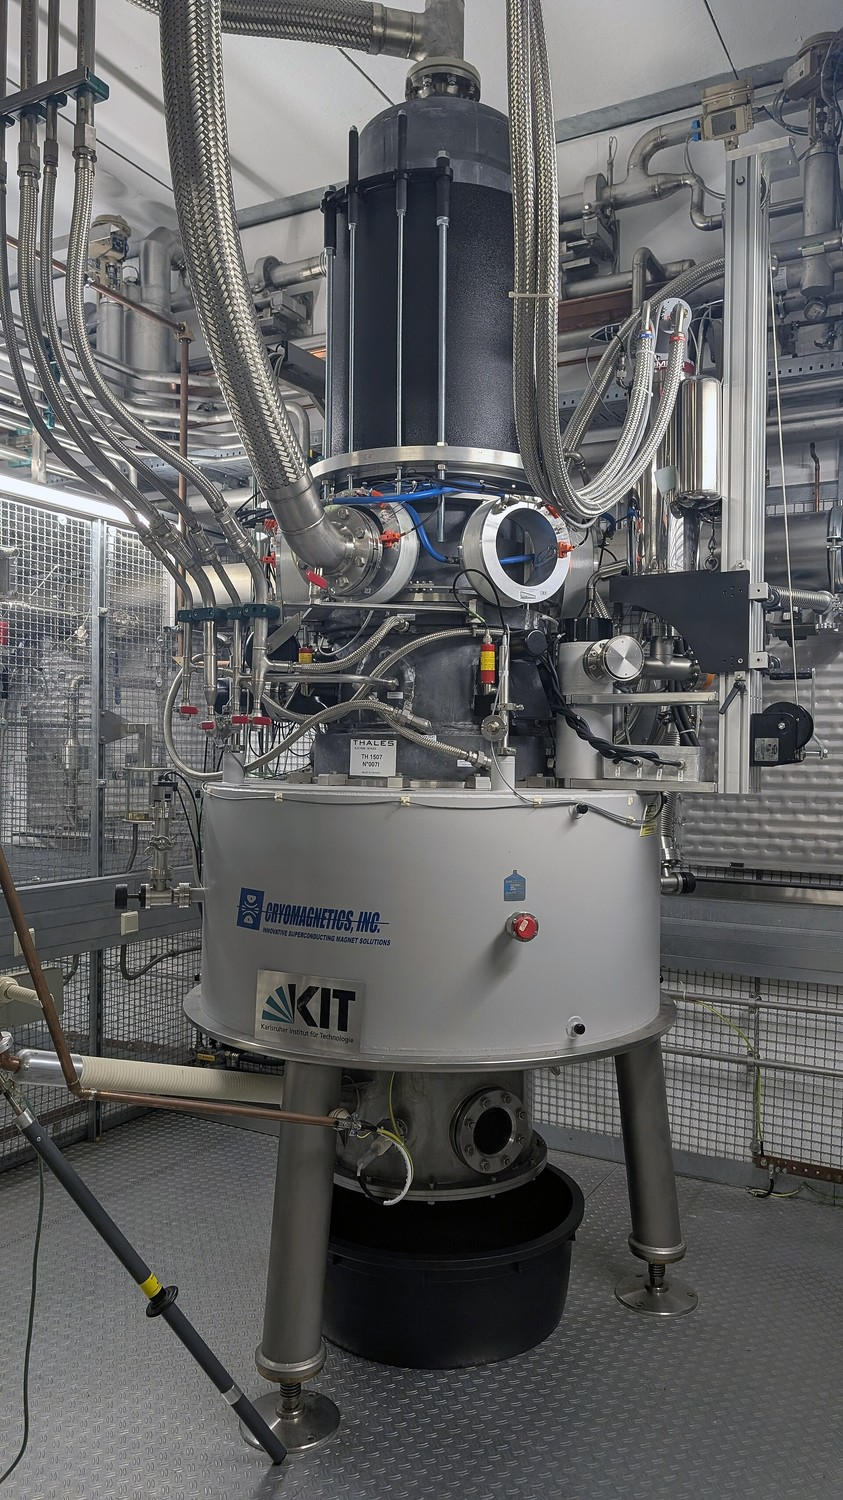
\includegraphics[width=0.78\textwidth]{../figures/gyrotron_ecrh.jpg}
\caption{回旋管：把波送进共振层的那台机器。电子回旋共振加热用的就是这种管子：它把微波功率送到 $\omega=\omega_{ce}$ 的共振层，波在截止与共振之间找到入口——本节算的加热落点，最终由这台机器对准。}
\label{fig:photo-appat2}
\figsource{Siarhei Besarab，CC BY-SA 4.0（Wikimedia Commons），链接见 figures/CREDITS.md。}
\end{figure}

\section{共振条件与加热落点：ECRH 与 ICRH 的坐标}
\label{sec:app-at-heating}

把「波在哪里被吸收」写成公式，就是共振条件。电子回旋加热用基频时要求

\begin{equation}
\omega=k_\parallel v_\parallel+\frac{n\omega_\mathrm{ce}}{\gamma}
\qquad (n=1,2,\dots),
\label{eq:app-at-icrh}
\end{equation}

其中 $n$ 是谐波数、$\gamma$ 是相对论因子、$k_\parallel v_\parallel$ 是多普勒项。
$k_\parallel=0$ 时它退化成 $\omega=n\omega_\mathrm{ce}$：$140$ GHz 的基频落在
$B=5.0$ T、即 $r=0.370237$ m；二次谐波要求 $B=2.50067$ T、对应 $r=6.94047$ m，在装置之外。
这就是「$140$ GHz 在这台装置上只能打基频」的算术原因。

离子回旋加热的频率要低三个数量级。在 $B_0=5.3$ T 下：

\begin{equation}
f_\mathrm{c}=\frac{ZeB}{2\pi m_\mathrm{i}}:\qquad
f_\mathrm{cH}=80.7995\ \mathrm{MHz},\quad
f_\mathrm{cD}=40.4088\ \mathrm{MHz},\quad
f_\mathrm{cHe3}=27.1291\ \mathrm{MHz}.
\label{eq:app-at-layers}
\end{equation}

取 $f_\mathrm{ICRH}=80.8$ MHz，则 H 基频层落在 $B=5.30003$ T（$r=-3.92696\times10^{-5}$ m，
几乎正好在轴上），D 二次谐波层落在 $B=5.29885$ T（$r=0.00134951$ m）。两层只差
$0.00138878$ m——这就是常见的「少数离子加热」构型：H 的基频与 D 的二次谐波几乎重合
（理想 $m_\mathrm{D}=2m_\mathrm{p}$ 时 $2f_\mathrm{cD}=80.8176$ MHz，与 $f_\mathrm{cH}$ 之比
$1.000223998$，只差万分之二）。

\begin{table}[htbp]
\centering
\small
\caption{加热方案的落点（D1 剖面，$140$ GHz 与 $80.8$ MHz）。}
\label{tab:app-at-heating}
\begin{tabular}{p{4.4cm}p{3.0cm}p{4.0cm}p{3.4cm}}
\hline
方案 & 条件 & 落点 & 备注 \\
\hline
寻常模基频 & $\omega=\omega_\mathrm{ce}$ & $r=0.370237$ m & $n_\mathrm{e0}<n_\mathrm{c}$，一路通行 \\
反常模基频 & 同左 & 被 $1.578$ m 反射 & 消逝带指数 $2792.83$ \\
二次谐波（反常） & $\omega=2\omega_\mathrm{ce}$ & $r=6.94047$ m & 在器壁之外 \\
上混杂共振 & $\omega=\omega_\mathrm{UH}$ & $r=1.31050$ m & 消逝带内端 \\
H 基频（ICRH） & $f_\mathrm{cH}=80.8$ MHz & $r=-3.92696\times10^{-5}$ m & 轴上 \\
D 二次谐波 & $2f_\mathrm{cD}=80.8$ MHz & $r=0.00134951$ m & 与 H 基频相差 $0.00138878$ m \\
\hline
\end{tabular}
\end{table}

\begin{tip}{加热位置由磁场和频率共同决定}{tip-app-at-heating}
「用哪个频率加热哪里」不是工程参数，而是 $B(r)$ 与谐波条件的交点：$\omega=n\omega_\mathrm{ce}(r)$。
磁场剖面一变，同一台加热系统的功率沉积位置就整体搬家——这就是为什么加热方案必须和
位形设计一起做。
\end{tip}

本节凡标出数字的量都由 \texttt{tmp/appAT\_calc.py} 复算。
\textbf{出处：}电子回旋与离子回旋共振条件、少数离子加热的谐波重合见 Wesson,
\emph{Tokamaks}（2011）第 11 章与 ITER Physics Basis（1999）第 6 章；本附录只做数值复算，
不复制原书表格与图。

\section{色散面与 CMA 图：把传播区域画成一张图}
\label{sec:app-at-cma}

截止与共振都是 $X$、$Y$ 平面里的曲线：寻常模截止是 $P=0$、反常模两个截止是 $R=0$ 与 $L=0$、
上混杂共振是 $S=0$。把 $X=\omega_\mathrm{pe}^2/\omega^2$、$Y=\omega_\mathrm{ce}/\omega$ 当坐标，
这些曲线把平面切成若干区域，每个区域里传播的模式与偏振是固定的——这就是 CMA 图。

\begin{equation}
P=0:\ X=1,\qquad
R=0:\ X=1+Y,\qquad
L=0:\ X=1-Y,\qquad
S=0:\ X=1-Y^2 .
\label{eq:app-at-cma}
\end{equation}

同一台装置在不同频率上就是图上的不同点。$n_\mathrm{e}=n_\mathrm{e0}$、$B=5.3$ T 时：

\begin{table}[htbp]
\centering
\small
\caption{同一介质在不同频率下的 CMA 坐标（$n_\mathrm{e}=n_\mathrm{e0}$、$B=5.3$ T）。}
\label{tab:app-at-cma}
\begin{tabular}{p{2.6cm}p{3.0cm}p{3.0cm}p{3.2cm}p{3.2cm}}
\hline
频率 & $X$ & $Y$ & $n_\mathrm{O}^2$ & $n_\mathrm{X}^2$ \\
\hline
$100$ GHz & $0.806164$ & $1.4836$ & $0.193836$ & $1.07785$ \\
$140$ GHz & $0.411308$ & $1.05972$ & $0.588692$ & $1.45317$ \\
$170$ GHz & $0.278949$ & $0.872707$ & $0.721051$ & $5.95813$ \\
$200$ GHz & $0.201541$ & $0.741801$ & $0.798459$ & $0.351618$ \\
\hline
\end{tabular}
\end{table}

表中 $n_\mathrm{X}^2$ 是垂直传播的值，只能说明「介质里有两个传播的模」；至于波从外面
能不能走到某个层，还要看沿路径有没有消逝带（第三节的算法）。CMA 图给的是\textbf{分类}，
不是\textbf{路径}——这一点在写程序时特别容易搞混：图上一个点在传播区，不代表天线发出的波
能走到那里。

\begin{tip}{CMA 图是分类，不是计算}{tip-app-at-cma}
CMA 图回答「这个频率上介质属于哪一类、有哪些模能存在」；它不回答「波能不能从器壁走到
第 5 节那个共振层」。后者要靠沿路径扫 $n^2$ 的符号，也就是第三节的做法。
\end{tip}

本节凡标出数字的量都由 \texttt{tmp/appAT\_calc.py} 复算。
\textbf{出处：}CMA 图的构造与各区域边界（$P=0$、$R=0$、$L=0$、$S=0$）见 Stix（1992）第 2 章
与 Swanson（2003）第 2 章；本附录不复制原图，只复算图中坐标。
\section{估算练习}
\label{sec:app-at-problems}

\textbf{练习 1}（CMA 坐标）把频率从 $140$ GHz 换成 $100$ GHz，密度与磁场不变。求 $X$、$Y$，
判断寻常模的截止密度还够不够用，并给出垂直传播的两个折射率平方。

\textbf{练习 2}（消逝层的厚度预算）某装置的消逝带里 $|n_\mathrm{X}|$ 的平均值是 $0.3$。
若要求波有 $1\%$ 的功率透过，这段消逝带最多能有多厚？如果 $|n_\mathrm{X}|$ 涨到 $0.5$ 或 $1$，
上限变成多少？

\textbf{练习 3}（伯恩斯坦波）电子伯恩斯坦波取 $k_\perp\rho_\mathrm{e}=0.3$。求它的频率、垂直波长与
群速度；再求「频率比上混杂高 $1$ GHz」对应的 $k_\perp$ 与垂直波长。

\textbf{练习 4}（离子伯恩斯坦波）同样的 $k_\perp\rho_\mathrm{i}=0.1$、$0.3$、$0.5$ 三档，
离子伯恩斯坦波的频率各是多少？垂直波长各是多少？

\textbf{练习 5}（少数离子加热）在 $B_0=5.3$ T 下求 H 与 D 的回旋频率，验证
$2f_\mathrm{cD}\approx f_\mathrm{cH}$ 的偏差；再求 $80.8$ MHz 时 H 基频层与 D 二次谐波层的
半径差。

\textbf{练习 6}（换频看剖面）把频率换成 $170$ GHz 与 $200$ GHz，求 $X$、$Y$ 与两个垂直折射率
平方，并说明为什么「$n_\mathrm{X}^2>0$」不等于「波能走到共振层」。

\textbf{解答 1} $X=(f_\mathrm{pe}/f)^2=0.806164$、$Y=f_\mathrm{ce}/f=1.4836$，
于是 $R=0.0812266$、$L=25.3636$、$S=12.7224$、$D=-12.6412$，
$n_\mathrm{O}^2=0.193836$、$n_\mathrm{X}^2=1.07785$。寻常模的截止密度还剩
$1/0.806164=1.24044$ 倍的余量：把中心密度提高两成四才会碰到寻常模截止。

\textbf{解答 2} 透过率 $T=\exp(-2k_0|n|L)=0.01$ 给出 $2k_0|n|L=\ln 100=4.60517$，
即 $L=\dfrac{4.60517}{2k_0|n|}$。$|n|=0.3$ 时 $L=2.61582$ mm；$0.5$ 时 $1.56949$ mm；
$1$ 时 $0.784745$ mm。本装置的消逝带厚 $0.267$ m，比最宽松的上限还厚一百多倍。

\textbf{解答 3} $k_\perp\rho_\mathrm{e}=0.3$ 给 $k_\perp=6954.33$ m$^{-1}$，
$f=189.777$ GHz（比上混杂高 $16.363$ GHz）、$\lambda_\perp=0.903492$ mm，
群速度 $v_\mathrm{g}=2.8293\times10^{7}$ m s$^{-1}$。频率高 $1$ GHz 只需要
$k_\perp=1682.44$ m$^{-1}$（$k_\perp\rho_\mathrm{e}=0.0725779$），对应
$\lambda_\perp=3.73458$ mm。

\textbf{解答 4} $k_\perp=34.3387$ m$^{-1}$ 时 $f=1.13836$ GHz；$103.016$ m$^{-1}$ 时
$1.13847$ GHz；$171.694$ m$^{-1}$ 时 $1.13869$ GHz。三档的频率差别只有万分之三，
因为它们都贴在下混杂频率（$1.13834$ GHz）上。

\textbf{解答 5} $f_\mathrm{cH}=80.7995$ MHz、$f_\mathrm{cD}=40.4088$ MHz，
所以 $2f_\mathrm{cD}=80.8176$ MHz，与 $f_\mathrm{cH}$ 之比 $1.000223998$——只差万分之二。
在 $80.8$ MHz 上，H 基频层落在 $r=-3.92696\times10^{-5}$ m、D 二次谐波层落在
$r=0.00134951$ m，两者相距 $0.00138878$ m：这就是「少数离子加热」把功率投在同一小片
等离子体上的算术依据。

\textbf{解答 6} $170$ GHz：$X=0.278949$、$Y=0.872707$、$n_\mathrm{O}^2=0.721051$、
$n_\mathrm{X}^2=5.95813$。$200$ GHz：$X=0.201541$、$Y=0.741801$、$n_\mathrm{O}^2=0.798459$、
$n_\mathrm{X}^2=0.351618$。两个频率上垂直传播都成立，但波从器壁走到共振层还要看路径：
$170$ GHz 时反常模同样要先过 $L$ 截止层，$n_\mathrm{X}^2>0$ 只说明「层本身不反射」，
不说明「能到达」。

\section{来源、分级与版权说明}
\label{sec:app-at-source}

本附录的推导与数值都定位在「冷等离子体线性波」这一层，不涉及非线性、不涉及输运、也不涉及
加热效率的工程核算（那三块分别属于附录 AL、AF 与 M）。所有频率、折射率、消逝带与隧穿指数
都由 \texttt{tmp/appAT\_calc.py} 按 D1 工作点复算，脚本随仓库发布。

\begin{table}[htbp]
\centering
\small
\caption{本附录的借鉴来源与使用方式。}
\label{tab:app-at-source}
\begin{tabular}{p{4.6cm}p{3.6cm}p{7.6cm}}
\hline
来源 & 用在哪一节 & 使用方式 \\
\hline
Stix, \emph{Waves in Plasmas}（1992）第 1--3 章 & 全篇 & 色散关系与 CMA 分类的知识框架；不复制原书表格与图 \\
Swanson, \emph{Plasma Waves}（2003）第 2--4 章 & 全篇 & 张量形式与截止/共振分类的对照；不复制原书图表 \\
Bernstein（1958）& 伯恩斯坦波一节 & 模式存在性与长波色散关系的原始文献；不复制原文公式编号 \\
Preinhaelter 与 Kopecky（1973）& 隧穿与 O--X--B & O--X 转换与隧穿处理的来源；只复算数值，不复制图表 \\
Laqua 等（1997）& 隧穿与 O--X--B & EBW 加热实验背景；不复制实验图 \\
Wesson, \emph{Tokamaks}（2011）第 11 章 & 加热落点 & 共振条件与加热方案的表述；不复制原书图 \\
ITER Physics Basis（1999）第 6 章 & 加热落点 & ECRH/ICRH 参数口径的对照；不复制原书表格 \\
\hline
\end{tabular}
\end{table}

本附录\textbf{不复制}任何原书的表格、图或习题；所有数字都是按本装置 D1 工作点重新计算的，
单位与有效位数按本套教材的统一口径给出。凡是直接沿用经典结论的地方（例如「基频反常模需从
高场侧发射」、「消逝带内透过率呈指数」），都在正文中写明出处，供读者自行核对。

\begin{tip}{本附录不给什么}{tip-app-at-honest}
本附录不给：加热效率与功率沉积剖面的自洽计算、非线性参量过程、动理学阻尼率、以及天线耦合
的工程细节。它只回答一个几何问题——波在哪里停、在哪里被吸收、中间那段消逝带有多厚。
其余问题属于附录 M（加热与电流驱动）、AL（非线性）与 AS（射线与波束）。
\end{tip}

本节凡标出数字的量都由 \texttt{tmp/appAT\_calc.py} 复算。
\textbf{出处：}来源分级与版权口径沿用本套教材的统一约定（只复算、不复制）；
参考文献的完整信息见 \texttt{README.md} 的「借鉴来源」一节。
